\section{Property-Based Test Corpus (\FVSpec:PBT)}
\Secl{dataset}

We scrape real-world Python property-based tests from public GitHub repositories that depend on Hypothesis~\cite{maciver2019hypothesis}. Our scraper operates in three stages.
\emph{(1) Discovery.} We crawl the Hypothesis dependency graph using PyGitHub~\cite{pygithub} and persist 19{,}808 unique \texttt{owner/repo} pairs into a static snapshot.
\emph{(2) Licensing.} We skip repositories with an explicitly non-permissive license (e.g.\ AGPL, GPL, LGPL, MPL), and record the license string---including ``unknown'' for repositories with no detectable license---alongside the rest of each repository's metadata.
\emph{(3) Extraction.} We shallow-clone each accepted repository, locate PBTs via \texttt{ripgrep}, and parse the surrounding Python to recover the transitive closure of locally-defined functions called therein.\footnote{We also scrape TypeScript PBTs written using \texttt{fast-check}~\cite{fastcheck}; however, we chose to scope our Lean extraction in this work to just the Python PBTs due to token budget. The TypeScript PBTs are included in our dataset for future use.}

A 24-hour run produced 54{,}345 raw PBTs.
The GitHub dependency graph surfaces many forks of the same upstream (e.g.\ hundreds of forks of \texttt{pytorch} carrying an identical Hypothesis suite), so we group repositories by base name, retain the most-starred ``canonical'' fork per group, and additionally drop tests whose whitespace-normalized SHA-256 already appears in the canonical set.
After deduplication the working corpus is 11{,}039 PBTs across 333 repositories owned by 281 distinct GitHub users, spanning 303 distinct upstream project names.

\subsection{Diversity}
\label{sec:dataset-diversity}

A perennial concern with scraped benchmarks is concentration: SWE-bench~\cite{jimenez2024swebench}, for instance, draws all 2{,}294 of its task instances from just 12 repositories, with \texttt{django} alone supplying 37\% and the top three (\texttt{django}, \texttt{sympy}, \texttt{scikit-learn}) supplying 64\%. Our corpus is far more spread out---it draws from 333 repositories, no single one of which contributes more than 8.7\% of the PBTs and whose top ten together contribute 58.5\%---and most of those repositories are unstarred personal projects rather than curated showcase code (Table~\ref{tab:dataset-stats}). The median PBT is just 13~LoC, but exercises around $3\times$ its own length in project code (see Figure~\ref{fig:pbt-vs-deps}).

To illustrate the diversity of our dataset, consider the result of drawing ten repositories from it uniformly at random:\footnote{Reproduce with \texttt{random.seed(13); random.sample([r for r in repos if r.stars >= 10], 10)} against the 333-repo deduplicated corpus; the star floor filters out personal forks.}
\texttt{sec-parser} (SEC-filings parser),
\texttt{whenever} (datetime library),
\texttt{LDAR\_Sim} (methane leak-detection simulator),
\texttt{bowtie} (JSON-schema test runner),
\texttt{Ivy-Octernships-ML} (ML-framework scaffolding),
\texttt{aaanalysis} (amino-acid analysis library),
\texttt{shrinkray} (test-case shrinker),
\texttt{logot} (log-output assertion library),
\texttt{tokenizations} (NLP tokenisation), and
\texttt{onnx-embedding} (ONNX-backed embedding library).
This is broadly representative of real-world software engineering, as opposed to purely academic or competitive programming.

Figure~\ref{fig:python_source} summarizes three code-quality metrics across the corpus.
The source tests span a wide range of complexity, from trivial single-assertion tests to multi-strategy tests exercising complex library APIs---diversity inherited directly from real-world engineering practice and not curated for difficulty.

\begin{figure}[t]
  \centering
  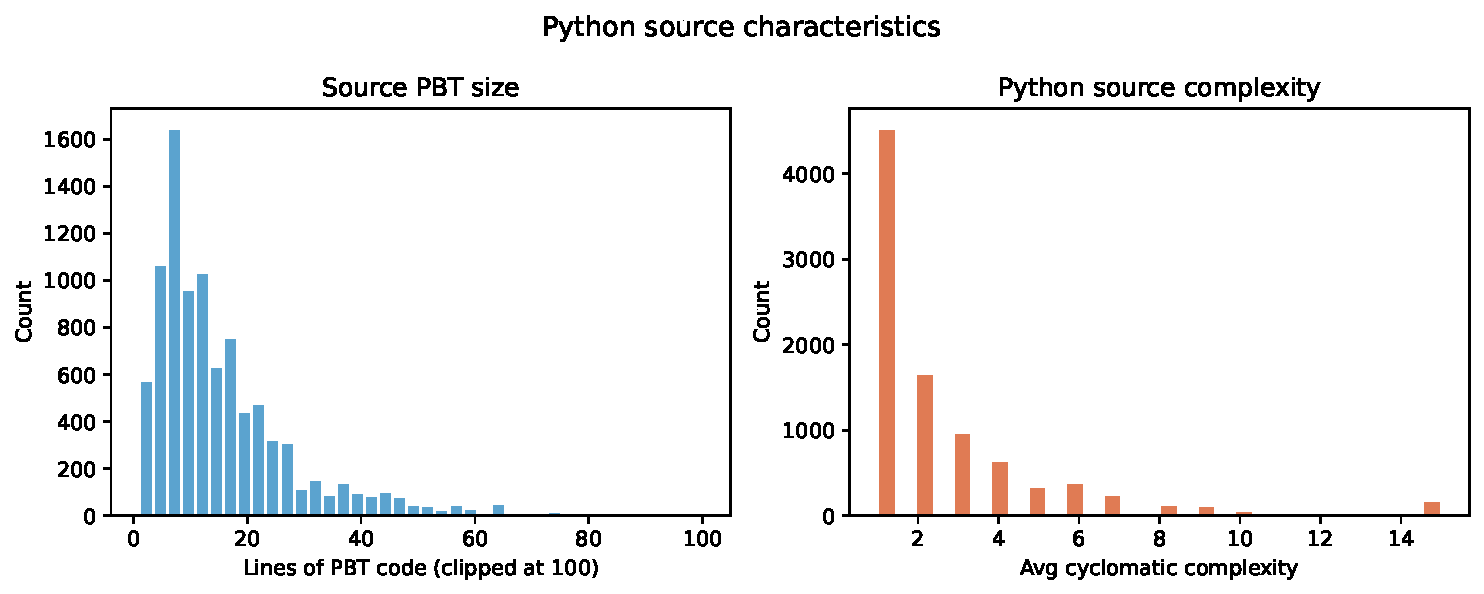
\includegraphics[width=\linewidth]{figs/python_source.pdf}
  \caption{Code-quality metrics for the 11{,}039 deduplicated PBTs, computed by Radon~\cite{radon}. \emph{Left}: lines of code.
  \emph{Center}: cyclomatic complexity---the number of linearly independent execution paths through the function, i.e.\ one plus the number of binary branch points~\cite{mccabe1976complexity}; higher values indicate more complex control flow.
  \emph{Right}: maintainability index---a 0--100 composite of Halstead volume~\cite{halstead1977elements}, cyclomatic complexity, and source lines, where higher is more maintainable; the spike at 100 is an artefact of Radon capping the score at that value.}
  \label{fig:python_source}
\end{figure}

\begin{figure}[t]
  \centering
  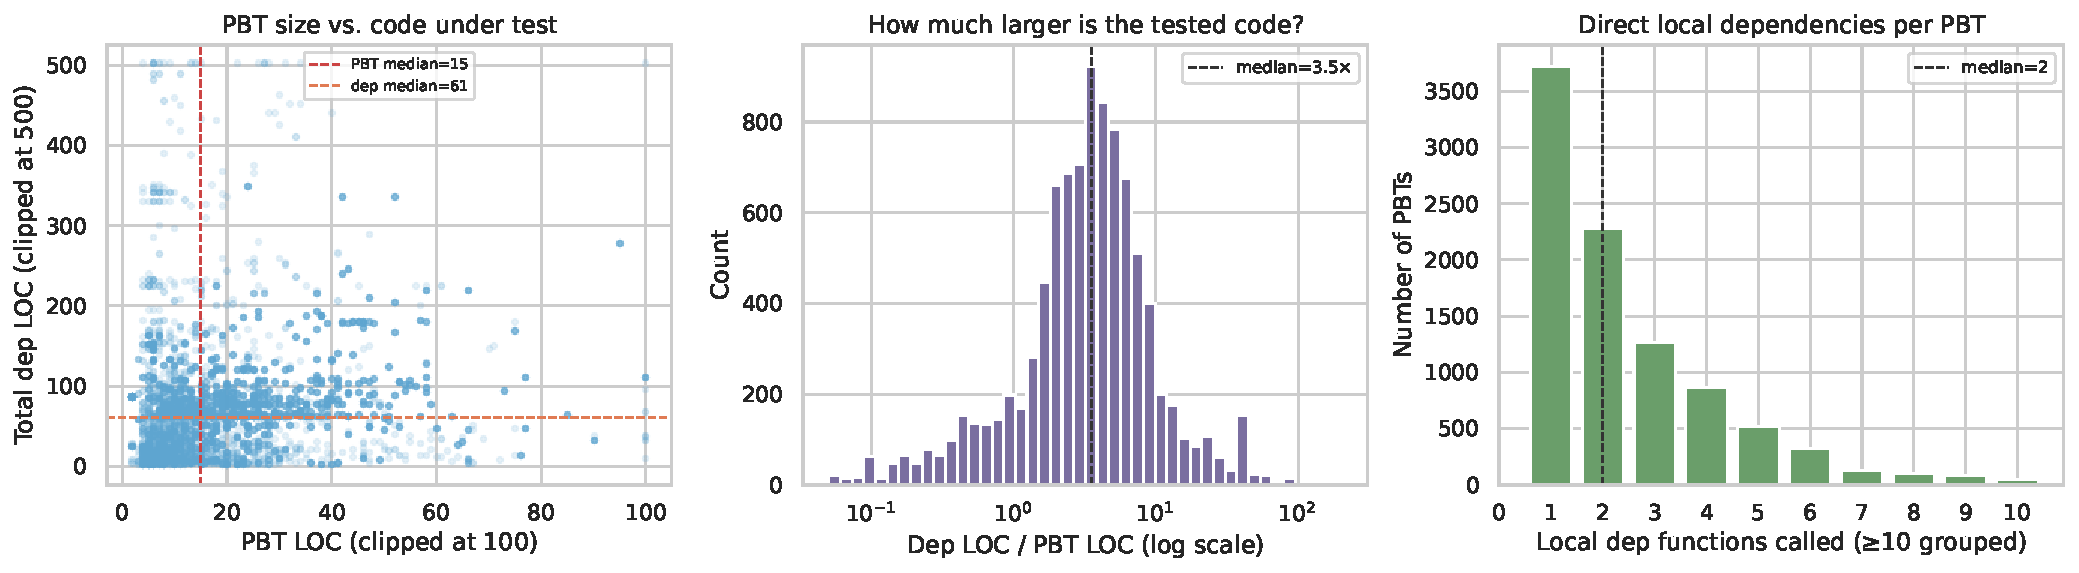
\includegraphics[width=\linewidth]{figs/realpbt_pbt_vs_deps.pdf}
  \caption{Three views of the relationship between PBT size and the size of the
  code being exercised, over the $n=6{,}912$ post-deduplication PBTs whose
  local dependencies were recoverable.
  (The remaining $4{,}127$ either exercise only standard-library or external code, or had dep extraction fail; the figure is therefore a subset of the full $11{,}039$-PBT corpus.)
  (a)~Per-PBT scatter of PBT LoC against the total LoC of the directly-called
  dependencies.
  (b)~Histogram of the ratio between dependency LoC and PBT LoC (log scale);
  the median PBT exercises code $3.3\times$ its own length.
  (c)~Histogram of the number of direct local function calls per PBT.}
\label{fig:pbt-vs-deps}
\end{figure}

\subsection{Comparison with the Hypothesis Corpus}
\label{sec:dataset-hc}

\begin{table}[t]
\centering
\begin{minipage}[t]{0.36\textwidth}
  \centering
  \caption{PBT corpus statistics.}
  \label{tab:dataset-stats}
  \footnotesize
  \begin{tabular}{lr}
    \toprule
    \textbf{Metric} & \textbf{Value} \\
    \midrule
    PBTs (raw scrape)              & 54{,}345 \\
    PBTs (post-dedup)              & 11{,}039 \\
    Unique repositories            & 333 \\
    Unique GitHub owners           & 281 \\
    Upstream project names         & 303 \\
    Top-1 / top-10 PBT share       & 8.7\% / 58.5\% \\
    \midrule
    \multicolumn{2}{@{}l}{\emph{Per-repo (min / med / max):}} \\
    PBTs per repo                  & 1 / 6 / 956 \\
    Stars                          & 0 / 0 / 9{,}438 \\
    Forks                          & 0 / 0 / 1{,}567 \\
    \midrule
    \multicolumn{2}{@{}l}{\emph{Per-PBT (min / med / max):}} \\
    PBT LoC                        & 2 / 13 / 174 \\
    Direct fn deps                 & 0 / 1 / 15 \\
    \bottomrule
  \end{tabular}
\end{minipage}\hfill
\begin{minipage}[t]{0.62\textwidth}
  \centering
  \setlength{\tabcolsep}{3pt}
  \caption{Comparison with HC-2026~\cite{devoe2026hypothesis}.}
  \label{tab:dataset-comparison}
  \footnotesize
  \begin{tabular}{@{}l c c@{}}
    \toprule
    & \textbf{\FVSpec:PBT} & \textbf{HC-2026} \\
    \midrule
    Discovery        & dep.\ graph        & GitHub search \\
    Raw PBTs         & 54{,}345           & 38{,}885 \\
    Tests (deduped)  & 11{,}039           & 23{,}139 \\
    Repos            & 333                & 1{,}504 \\
    Repo dedup       & fork/name          & \texttt{is\_fork} \\
    Test dedup       & SHA-256            & parametrization \\
    License filter   & no copyleft        & none \\
    Per-test data    & source + metrics   & runtime + coverage \\
    \midrule
    Repo overlap (valid)  & \multicolumn{2}{c}{28 / 333 \enskip(8\%)} \\
    Repo overlap (any)    & \multicolumn{2}{c}{111 / 333 \enskip(33\%)} \\
    \bottomrule
  \end{tabular}
\end{minipage}
\end{table}

While we were finalizing this work, the Hypothesis maintainers released their own scraped corpus~\cite{devoe2026hypothesis} (HC-2026).
The two corpora target different downstream uses---HC-2026 is built to study Hypothesis \emph{runtime} behavior (entropy consumption, predicate firing, coverage), while ours is built to feed a Lean formalization pipeline---which drives the design differences summarized in Table~\ref{tab:dataset-comparison}.
A consequence of HC-2026's runtime focus is that it filters out as ``invalid'' any repository whose PBTs may not be directly runnable without some custom setup: code that depends on external services, API keys, environment variables, or live databases. Our pipeline imposes no such requirement, since we only need a PBT's source code to translate it into Lean. Of our 333 repositories, 28 appear in HC-2026's valid (executable) set and 111 (33\%) appear in the pre-validity superset---meaning roughly 80 of our repositories were dropped by HC-2026 for being too operationally entangled to run, consistent with our goal of producing challenging and realistic FV problems.
Future work could merge the two corpora to enlarge the input pool; we did not pursue this here because the present token budget does not exhaust even our own 11{,}039-PBT corpus.

Next, we describe the pipeline by which we transpile our PBT corpus into Lean FV challenges.
